\documentclass[a4paper,12pt]{article}
\usepackage[utf8]{inputenc}
\usepackage{amsmath, subcaption, amssymb, graphicx, booktabs, pgfplots, pgfplotstable, float}
\usepackage{geometry}
\geometry{left=2cm, right=2cm, top=2.5cm, bottom=2.5cm}
\renewcommand{\figurename}{Figura}
\renewcommand{\tablename}{Tabla}

\title{Relación de Problemas 1: Variables Estadísticas Unidimensionales}
\author{Salvador Gil Antonio \and Salvador Gil Sergio \and Serantes Rivas Víctor\\\\Estadística Descriptiva e Introducción a la Probabilidad \\ Primer curso del Doble Grado en Ingeniería Informática y Matemáticas}
\date{}

\begin{document}

\maketitle
\section*{Ejercicio 1} El número de hijos de las familias de una determinada barriada de una ciudad es una variable estadística de la que se conocen los siguientes datos: 

\begin{center}
    \begin{tabular}{c|c|c|c}
        $x_i$ & $n_i$ & $N_i$ & $f_i$ \\
        \hline
        0 & 80 & - & 0.16 \\
        1 & 110 & - & - \\
        2 & - & 320 & - \\
        3 & -  & - & 0.18 \\
        4 & 40 &  - & - \\
        5 & -  & - & - \\
        6 & 20 &  - & -\\
    \end{tabular}
\end{center}

(a) Completar la tabla de frecuencias.\\
\begin{center}
    \begin{tabular}{c|c|c|c}
        $x_i$ & $n_i$ & $N_i$ & $f_i$ \\
        \hline
        0 & 80 & 80 & 0.16 \\
        1 & 110 & 190 & 0.22  \\
        2 & 130 & 320 & 0.26  \\
        3 & 90 & 410  & 0.18 \\
        4 & 40 & 450 & 0.08  \\
        5 & 30 & 480 & 0.06  \\
        6 & 20 & 500 & 0.04  \\
    \end{tabular}
\end{center}

(b) Representar la distribución mediante un diagrama de barras y la curva de distribución.\\

\begin{figure}[H]
    \centering
    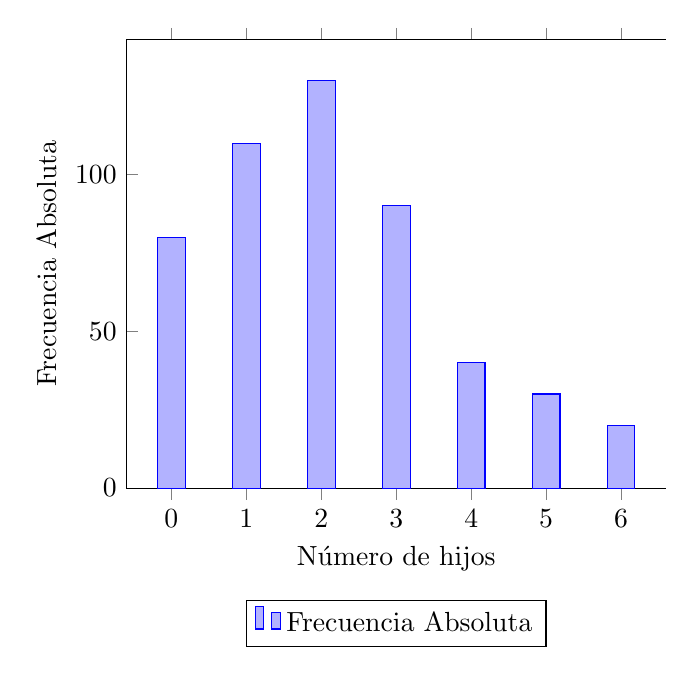
\begin{tikzpicture}
        \begin{axis}[
            ybar,
            axis y line*=left,
            symbolic x coords={0,1,2,3,4,5,6},
            xtick=data,
            ymin=0,
            ylabel={Frecuencia Absoluta},
            xlabel={Número de hijos},
            legend style={at={(0.5,-0.25)}, anchor=north, legend columns=-1}
        ]
        \addplot coordinates {(0,80) (1,110) (2,130) (3,90) (4,40) (5,30) (6,20)};
        \addlegendentry{Frecuencia Absoluta}
        \end{axis}
    \end{tikzpicture}
    \caption{Diagrama de barras }
\end{figure}

\begin{figure}[H]
    \centering
    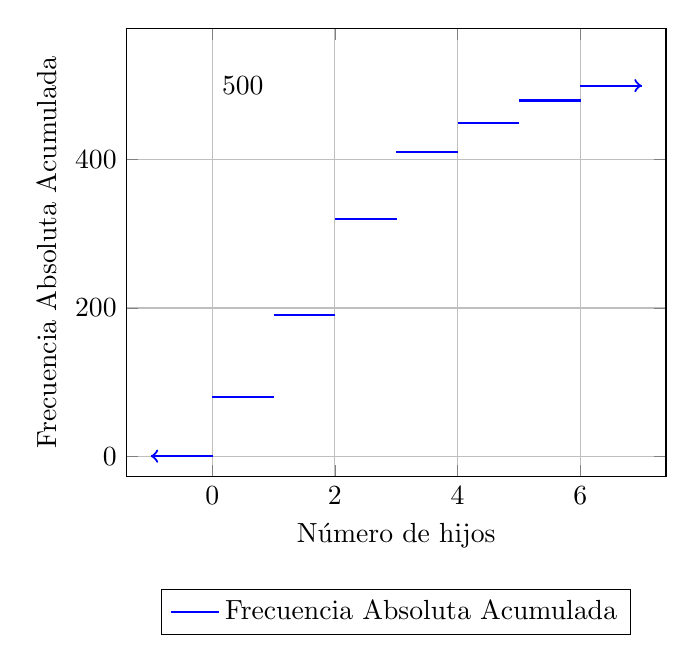
\begin{tikzpicture}
        \begin{axis}[
            xlabel={Número de hijos},
            ylabel={Frecuencia Absoluta Acumulada},
            ymin=0,
            ymax=550,
            grid=major,
            enlargelimits=0.05,
            legend style={at={(0.5,-0.25)}, anchor=north, legend columns=-1}
        ]
        \addplot[color=blue, mark=none, smooth][domain=-1:0,          samples=100, thick] {0};
        \addplot[color=blue, mark=none, smooth][domain=0:1,          samples=100, thick] {80};
        \addplot[color=blue, mark=none, smooth][domain=1:2,          samples=100, thick] {190};
        \addplot[color=blue, mark=none, smooth][domain=2:3,          samples=100, thick] {320};
        \addplot[color=blue, mark=none, smooth][domain=3:4,          samples=100, thick] {410};
        \addplot[color=blue, mark=none, smooth][domain=4:5,          samples=100, thick] {450};
        \addplot[color=blue, mark=none, smooth][domain=5:6,          samples=100, thick] {480};
        \addplot[color=blue, mark=none, smooth][domain=6:7,          samples=100, thick] {500};
        
        \draw[->, color=blue, mark=none, smooth, thick] (axis cs:0,0) -- (axis cs:-1,0);
        \draw[->, color=blue, mark=none, smooth, thick] (axis cs:6,500) -- (axis cs:7,500);
        
        \node at (axis cs:0,500) [anchor=west] {500};
        \addlegendentry{Frecuencia Absoluta Acumulada}
        \end{axis}
    \end{tikzpicture}
    \caption{Curva de distribución acumulada}
\end{figure}



(c) Calcular medidas de tendencia central e interpretar.

Las medidas de tendencia central que vamos a calcular son:
\begin{itemize}
    \item Media Aritmética: Dentro de la variable estadística "Número de Hijos" la media más apropiada es la aritmética, que indica el número de hijos que corresponde a cada individuo de la población (Cada familia de la barriada) si repartimos equitativamente el número total de Hijos ($N$ = 500)
\begin{center} 
    $$\bar x = \frac {1}{n} \sum\limits_{i = 1}^k {x_i n_i} = \frac {1070}{500} = 2.14$$
    
\end{center}
hay una media de 2.14 hijos por familia.

    \item Mediana: El valor de la modalidad recogida en la posición central de la distribución
    $$Me = x_i : N_{i-1} < \frac {n}{2} \leq N_i$$
    lo cuál, en esta distribución es: $$Me = 2$$
    Esto significa que si tomamos la mitad de individuos con el menor número de hijos, la mayor modalidad registrada entre ellos será 2, es decir, el 2 "deja por encima a la mitad superior de la distribución".

    \item Moda: Es la modalidad que más frecuencia absoluta registra de las observadas, es decir, la modalidad que más individuos presentan de entre los que se han observado. En esta distribución, la moda es:
    $$Mo = x_3 = 2$$ con $$n_3 = 130 \geq n_i \forall i = 1,...,7$$
\end{itemize}


\section*{Ejercicio 2} La puntuación obtenida por 50 personas que se presentaron a una prueba de selección, sumadas las puntuaciones de los distintos tests, fueron :

\begin{quote}
174, 185, 166, 176, 145, 166, 191, 175, 158, 156, 156, 187, 162, 172, 197, 181, 151, 161, 183, 172, 162, 147, 178, 176, 141, 170, 171, 158, 184, 173, 169, 162, 172, 181, 187, 177, 164, 171, 193, 183, 173, 179, 188, 179, 167, 178, 180, 168, 148, 173.
\end{quote}

(a) Agrupar los datos en intervalos de amplitud 5 desde 140 a 200 y construir la tabla de frecuencias.\\
\begin{center}
    \begin{tabular}{c|c|c|c}
        I & $n_i$ & $f_i$ & $N_i$ \\
        \hline
         (140,145] & 2 & 0.04 & 2 \\
         (145,150] & 2 & 0.04 & 4 \\
         (150,155] & 1 & 0.02 & 5 \\
         (155,160] & 4 & 0.08 & 9 \\
         (160,165] & 5 &  0.1 & 14 \\
         (165,170] & 6 & 0.12 & 20\\
         (170,175] & 10 &  0.2  & 30\\
         (175,180] & 8 &  0.16 & 38\\
         (180,185] & 6 &  0.12 & 44\\
         (185,190] & 3 &  0.06 & 47\\
         (190,195] & 2 &  0.04 & 49\\
         (195,200] & 1 &  0.02 & 50\\
    \end{tabular}
\end{center}


(b) Representar la distribución mediante un histograma, poligonal de frecuencias y curva de distribución.

\begin{figure}[H]
\centering
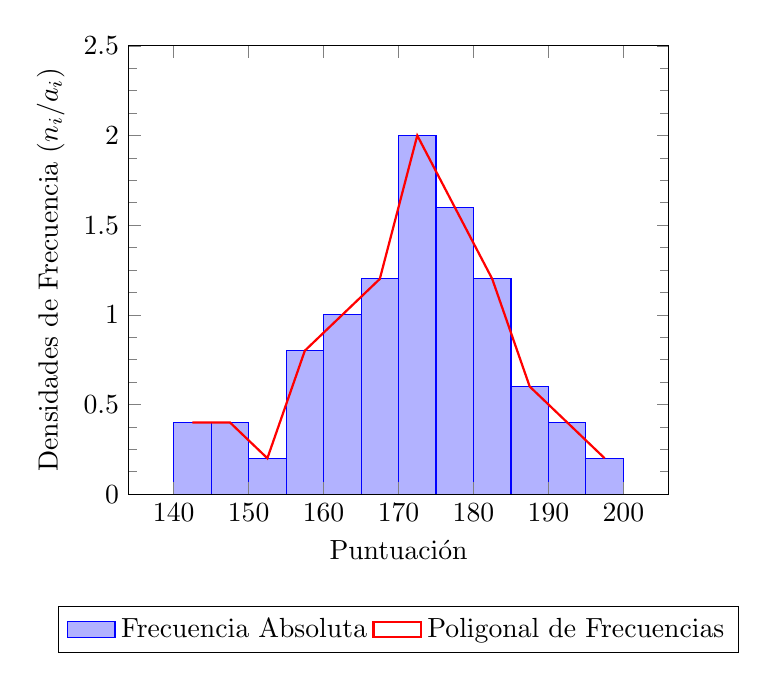
\begin{tikzpicture}
    \begin{axis}[
        xlabel={Puntuación},
        ylabel={Densidades de Frecuencia ($n_i$/$a_i$)},
        ymin=0, ymax=2.5,
        minor y tick num = 3,
        area style,
        legend style={at={(0.5,-0.25)}, anchor=north, legend columns=-1}
        ]
        \addplot+[ybar interval,mark=no] plot coordinates { (140,2/5) (145,2/5) (150,1/5) (155,4/5) (160,5/5) (165,6/5) (170,10/5) (175,8/5) (180,6/5) (185,3/5) (190,2/5) (195,1/5) (200,0) };
        \addlegendentry{Frecuencia Absoluta}
    
        
        \addplot[color=red, mark=none, thick] coordinates {(142.5,2/5) (147.5,2/5) (152.5,1/5) (157.5,4/5) (162.5,5/5) (167.5,6/5) (172.5,10/5) (177.5,8/5) (182.5,6/5) (187.5,3/5) (192.5,2/5) (197.5,1/5)
        };
        \addlegendentry{Poligonal de Frecuencias}
    \end{axis}

\end{tikzpicture}
\caption{Histograma y Poligonal de frecuencias}
\end{figure}

\begin{figure}[H]
    \centering
    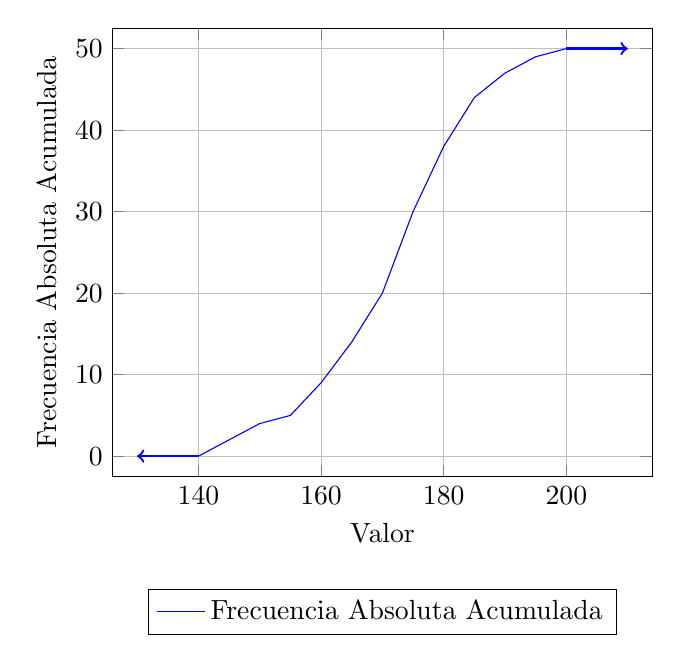
\begin{tikzpicture}
        \begin{axis}[
            ylabel={Frecuencia Absoluta Acumulada},
            xmin=130, xmax=210, % Ajusta los límites del eje x
            ymin=0, ymax=50,    % Ajusta los límites del eje y
            grid=major,
            enlargelimits=0.05,
            legend style={at={(0.5,-0.25)}, anchor=north, legend columns=-1},
            xlabel={Valor}
        ]
            % Curva de distribución acumulada
            \addplot[color=blue, mark=none] coordinates {
                (130, 0)(140, 0)(145, 2)(150, 4)(155, 5)(160, 9)(165, 14)
                (170, 20)(175, 30)(180, 38)(185, 44)(190, 47)(195, 49)(200, 50)(210, 50)
            };
            \addlegendentry{Frecuencia Absoluta Acumulada}

            % Flecha que va desde (130,0) hacia la izquierda
            \draw[->, color=blue, thick] (axis cs:140,0) -- (axis cs:130,0);

            % Flecha que va desde (200,50) hacia la derecha
            \draw[->, color=blue, thick] (axis cs:200,50) -- (axis cs:210,50);
        \end{axis}
    \end{tikzpicture}
    \caption{Curva de distribución acumulada}
\end{figure}

\section*{Ejercicio 3}
La distribución de la renta familiar en el año 2003 por comunidades autónomas se recoge en la siguiente tabla:

\begin{center}
    \begin{tabular}{|c|c|c|c|c|c|c|c|}
        \hline
        $I_i$ & $n_i$ & $N_i$ & $f_i$ & $F_i$ & $c_i$ & $a_i$ & $h_i$ \\
        \hline
        (8300, 9300] & 2 & - & - & - & - & - & - \\
        , 10200] & - & 5 & - & - & - &  & - \\
        - & - & - & - & 10/18 & - & 1100 & - \\
        - & - & - & 2/18 & - & 12000 & - & - \\
        - & 4 & - & - & - & - & - & 0.005/18 \\
        - & - & 18 & - & - & - & - & 0.002/18 \\
        \hline
    \end{tabular}
\end{center}

\begin{itemize}
    \item[a)] Completar la tabla.

\begin{center}
    \begin{tabular}{|c|c|c|c|c|c|c|c|}
        \hline
        $I_i$ & $n_i$ & $N_i$ & $f_i$ & $F_i$ & $c_i$ & $a_i$ & $h_i$ \\
        \hline
        (8300, 9300] & 2 & 2 & 2/18 & 2/18 & 8800 & 1000 & 0.002/18 \\
        (9300, 10200] & 3 & 5 & 3/18 & 5/18 & 9750 & 900 & 1/5400 \\
        (10200, 11300] & 5 & 10 & 5/18 & 10/18 & 10750& 1100 & 1/3960 \\
        (11300, 12700] & 2 & 12 & 2/18 & 12/18 & 12000 & 1400 & 1/12600 \\
        (12700, 13700] & 4 & 16 & 4/18 & 16/18 & 13200 & 1000 & 0.005/18 \\
        (13700, 14700] & 2 & 18 & 2/18 & 1 & 14200 & 1000 & 0.002/18 \\
        \hline
    \end{tabular}
\end{center}
    
    \item[b)] Representar la distribución mediante un histograma, poligonal de frecuencias y curva de distribución.

\begin{figure}[H]
\centering
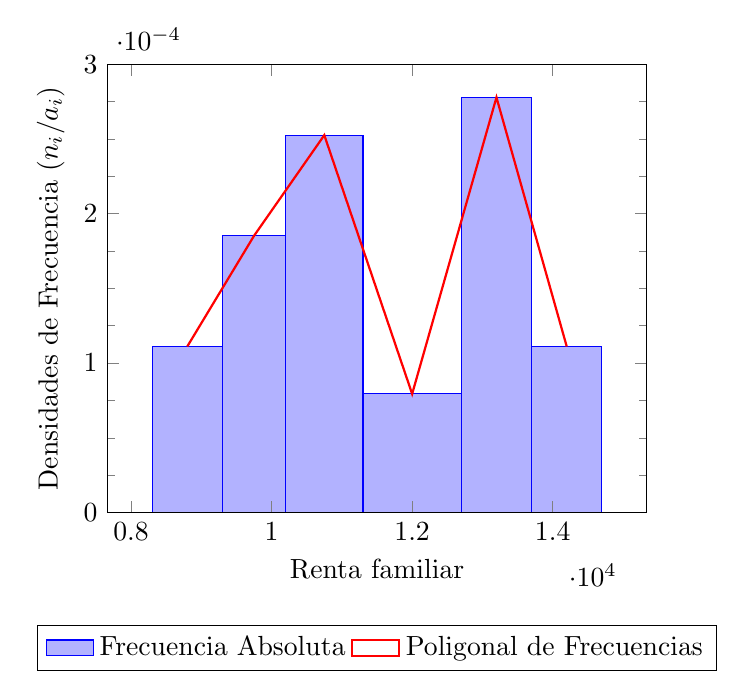
\begin{tikzpicture}
    \begin{axis}[
        xlabel={Renta familiar},
        ylabel={Densidades de Frecuencia ($n_i$/$a_i$)},
        ymin=0, ymax=0.0003,
        minor y tick num = 3,
        area style,
        legend style={at={(0.5,-0.25)}, anchor=north, legend columns=-1}
        ]
        \addplot+[ybar interval,mark=no] plot coordinates { (8300,0.002/18) (9300,1/5400) (10200,1/3960) (11300,1/12600) (12700,0.005/18) (13700,0.002/18) (14700,0) };
        \addlegendentry{Frecuencia Absoluta}
    
        
        \addplot[color=red, mark=none, thick] coordinates {(8800,0.002/18) (9750,1/5400) (10750,1/3960) (12000,1/12600) (13200,0.005/18) (14200,0.002/18)
        };
        \addlegendentry{Poligonal de Frecuencias}
    \end{axis}
\end{tikzpicture}
\end{figure}


\begin{figure}[H]
    \centering
    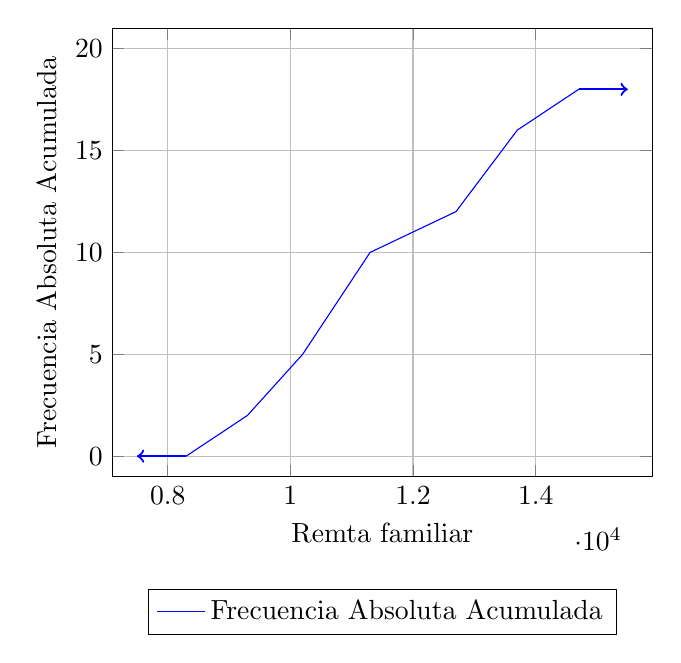
\begin{tikzpicture}
        \begin{axis}[
            ylabel={Frecuencia Absoluta Acumulada},
            xmin=7500, xmax=15500, % Ajusta los límites del eje x
            ymin=0, ymax=20,    % Ajusta los límites del eje y
            grid=major,
            enlargelimits=0.05,
            legend style={at={(0.5,-0.25)}, anchor=north, legend columns=-1},
            xlabel={Remta familiar}
        ]
            % Curva de distribución acumulada
            \addplot[color=blue, mark=none] coordinates {
                (7500, 0) (8300,0) (9300, 2) (10200, 5) (11300, 10) (12700, 12) (13700, 16) (14700, 18) (15500, 18)
            };
            \addlegendentry{Frecuencia Absoluta Acumulada}

            % Flecha que va desde (130,0) hacia la izquierda
            \draw[->, color=blue, thick] (axis cs:8300,0) -- (axis cs:7500,0);

            % Flecha que va desde (200,50) hacia la derecha
            \draw[->, color=blue, thick] (axis cs:14700,18) -- (axis cs:15500,18);
        \end{axis}
    \end{tikzpicture}
    \caption{Curva de distribución acumulada}
\end{figure}


    \item[c)] ¿Cuántas comunidades presentan una renta menor o igual que 12700 euros? ¿Y cuántas superior a 11300 euros?
    
    Para encontrar el número de comunidades con una renta menor o igual que 12700 euros, debemos encontrar la frecuencia absoluta acumulada que corresponde a esta cantidad. El intervalo (11300, 12700] $N_i$ = 12; por tanto, la respuesta es que hay un total de 12 comunidades con renta menor o igual a 12700 euros.

    La siguiente pregunta pide el número de comunidades con una renta superior a 11300 euros. Como la frecuencia absoluta acumulada para el intervalo $I_3$ = (10200, 11300] es $N_3$ = 10, entonces existen 10 comunidades con renta menor o igual que 11300 euros. Por tanto, para encontrar las comunidades con renta mayor a  11300 euros debemos restar el total de comunidades a $N_3$:
\begin {center}
    \begin{tabular}{}
   $N$ - $N_3$ = 18 - 10 = 8
    \end{tabular}
\end {center} 
    Hay 8 comunidades con renta superior a 11300 euros
    
\end{itemize}

\section*{Ejercicio 4}
En una determinada empresa se realiza un estudio sobre la calidad de su producción. La distribución siguiente informa sobre el número de piezas defectuosas encontradas en 100 cajas examinadas con 50 unidades cada una de ellas:

\begin{center}
    \begin{tabular}{|c|c|}
        \hline
        No piezas defectuosas & No de cajas \\
        \hline
        0 & 6 \\
        1 & 9 \\
        2 & 10 \\
        3 & 11 \\
        4 & 14 \\
        5 & 16 \\
        6 & 16 \\
        7 & 9 \\
        8 & 4 \\
        9 & 3 \\
        10 & 2 \\
        \hline
    \end{tabular}
\end{center}

\begin{itemize}
    \item[a)] Calcular el número medio de piezas defectuosas por caja.
    \item[b)] ¿Cuántas piezas defectuosas se encuentran más frecuentemente en las cajas examinadas?
    \item[c)] ¿Cuál es el número mediano de piezas defectuosas por caja?
    \item[d)] Calcular los cuartiles de la distribución. Interpretarlos.
    \item[e)] Calcular los deciles de orden 3 y 7. Interpretarlos.
    \item[f)] Cuantificar la dispersión de la distribución utilizando diferentes medidas, interpretando los resultados y señalando las ventajas e inconvenientes de cada una.
\end{itemize}

\\El problema da una población de número de piezas defectuosas por caja (de 0 a 10), con la variable estadística siendo el número de cajas que presentan dicho número de piezas defectuosas.\\

\begin{center}
    \begin{tabular}{|c|c|c|c|c|c|c|}
        \hline
        $x_i$ & $n_i$  & $N_i$ & $x_i n_i$ & $n_i |x_i - \bar x|$ & $n_i |x_i - Me|$ & $n_i (x_i - \bar x)^2$\\
        \hline
        0 & 6 & 6 & 0 & 26,16 & 27 & 114,057 \\
        1 & 9 & 15 & 9 & 30,24 & 31,5 & 101,606 \\
        2 & 10 & 25 & 20 & 23,6 & 25 & 55,696 \\
        3 & 11 & 36 & 33 & 14,96 & 16,5 & 20,395\\
        4 & 14 & 50 & 56 & 5,04 & 7 & 1,814\\
        5 & 16 & 66 & 80 & 10,24 & 8 & 6,553\\
        6 & 16 & 82 & 96 & 26,24 & 24 & 43,033\\
        7 & 9 & 91 & 63 & 23,76 & 22,5 & 62,726\\
        8 & 4 & 95 & 32 & 14,56 & 14 & 52,998\\
        9 & 3 & 98 & 27 & 13,92 & 13,5 & 64,588\\
        10 & 2  & 100 & 20 & 11,28 & 11 & 63,619\\
        \hline
        & 100 & & 436 & 200 & 200 & 587,035 \\
        \hline
    \end{tabular}
\end{center}

\begin {itemize}
    \item [a)]  
\end {itemize}

Para calcular el número de piezas defectuosas por caja simplemente realizamos la media aritmética: \\

    $\bar x$ = $\frac {1}{n} $\sum\limits_{i = 1}^k {x_i n_i}$ = $\frac{1}{100}*436$ = 4,36 piezas defectuosas$

\begin {itemize}
    \item [b)]  
\end {itemize}

    Este apartado nos pide calcular la moda de esta distribución. Rápidamente, podemos observar que es una distribución bimodal, cuya moda recae en los valores 5 y 6 de piezas defectuosas, que presentan 16 cajas cada uno.

\begin {itemize}
    \item [c)]  
\end {itemize}

    Ahora tenemos que calcular la mediana de la distribución. Primero comprobamos si hay algún valor de piezas defectuosas que tenga una frecuencia absoluta acumulada de $\frac {N}{2} = 50$, (o alternativamente una frecuencia relativa acumulada de $\frac{F}{2} = 0,5$), y encontramos que para $x_i = 4$, esto se cumple, lo que significa que cualquier número del intervalo $[4,5)$ tiene esa misma frecuencia absoluta acumulada, por lo que se hace la media aritmética entre el valor que lo cumple (4), y el inmediatamente superior (5), por lo que $Me= \frac{4+5}{2} = 4,5$ piezas defectuosas.

\begin {itemize}
    \item [d)]  
\end {itemize}

Hay un cuartil que ya hemos calculado, que es $Q_2 = Me = 4,5$ piezas. Esto significa que el 50\% de los datos observados en la distribución, es decir, la mitad de las cajas, presentan 4,5 piezas defectuosas o menos. \\
Para calcular $Q_1$, repetimos el proceso realizado para hayar la mediana, pero ahora con el valor que corresponde a $\frac{1}{4}N=25$, y vemos que tambien existe un valor de piezas defectuosas, $x_2 = 2$ piezas, que cumple que $N_2 = \frac{1}{4}N = 25$, lo que, realizando el mismo procedimiento que en la mediana, significa que $Q_1=2,5$ piezas defectuosas. Al igual que en el caso de la mediana, podemos interpretar esto como que el 25\% de las cajas presentan 2,5 piezas defectuosas o menos.\\
Finalmente, para calcular $Q_3$, repetimos el proceso con el valor $\frac{3}{4}N = 75$. En este caso, como podemos observar, no hay ningun valor en la distribución que cumpla que $N_i = \frac{3}{4}N$. Por el contrario, ahora esta frecuencia acumulada se encuentra entre los valores 5 y 6 de piezas defectuosas, por lo que $Q_3$ toma el valor del inmediatamente superior: $Q_3= 6$. Al igual que en los demás casos, esto nos cuenta que el 75\% de las cajas presentan 6 piezas defectuosas o menos (o alternativamente, que el 25\% de las cajas presentan más de 6 piezas defectuosas). \\

\begin {itemize}
    \item [e)]  
\end {itemize}

Para calcular los deciles de orden 3 y 7, realizamos el mismo procedimiento que en los dos apartados anteriores:\\

Para $D_3$, el decil de orden 3, observamos que no existen ningún valor que cumple que su frecuencia absoluta acumulada sea igual a $\frac{3}{10}N = 30$, por lo que el valor de $D_3$ equivale al que tiene $N_i$ inmediatamente superior a 30, que corresponde a $N_3 = 36$, por lo que $D_3 = 3$ piezas defectuosas. Esto significa que el 30\% de las cajas presentan 3 piezas defectuosas o menos.\\
En el caso de $D_7$ ocurre exactamente lo mismo, ya que $\frac{7}{10}N = 70$ y no existe ningun valor que tenga una frecuencia absoluta acumulada de 70 cajas, por lo que $D_7$ será el valor inmediatamente superior a 70, que lo toma $N_6 = 82$, por lo que el decil de orden 7 de la distribución será $D_7 =6$ piezas defectuosas. Exactamente igual a los casos anteriores, esto equivale a que 7 de cada 10 cajas presentan 6 piezas defectuosas o menos.\\ \\ 

\begin {itemize}
    \item [f)]  
\end {itemize}

Recorrido: $R=10 - 0 = 10$. Esto significa que la diferencia entre la caja que tiene más piezas defectuosas (10) y la que menos (0) es de 10 piezas.\\
Recorrido intercuartílico: $R_I = Q_3 - Q_1 = 6-2,5 = 3,5$. Es la longitud del intervalo que conforma el 50\% central de los datos, es decir, la distancia entre el número de cajas (2,5) que deja a la izquierda el 25\% inferior de los datos, y el número de cajas (6) que deja a la derecha el 25\% de los datos es de 3,5.\\
Desviación absoluta media respecto a la media: $D_\bar x$ = $\frac{1}{n}\sum\limits_{i = 1}^k ni|x_i - \bar x|$ = 2 piezas. Esto nos dice que, de media, los valores de piezas defectuosas por caja van a distar dos piezas defectuosas de la media, que es de 4,36 piezas\\
Desviación absoluta media respecto a la mediana: $D_{Me}$ = $D_\bar x$ = $\frac{1}{n}\sum\limits_{i = 1}^k ni|x_i - Me|$ = 2 piezas. Esto da a entender que la distancia media de los valores de piezas defectuosas de las cajas respecto de la media es de 2.\\
Varianza: $\sigma^2$= $\frac{1}{n}\sum\limits_{i=1}^kn_i(x_i-\bar x)^2$ = 5,87035 piezas. Es la media de la suma de las áreas de los cuadrados cuyo lado es la diferencia de los datos respecto de la media.\\
Desviación típica: $\sigma=+\sqrt{\sigma^2}$ = 2,4228, que representa la suma de los lados de los cuadrados que conforman la varianza.\\
Coeficiente de variación Pearson: $C.V.=\frac{\sigma}{\bar x}$= 0,5557. Esta medida es un coeficiente relativo, lo que significa que es ideal para comparar dos distribuciones aunque sus datos sean radicalmente distintos. Sirve para medir la dispersión respecto de la media, por lo que tiene todos los inconvenientes asociados a la misma.\\
Índice de dispersión respecto a la mediana: $V_{Me}= \frac{D_{Me}}{Me}=0,4444$. Esta medida tambien es una medida relativa de dispersión, por lo que tambien es muy útil al comparar dos distribuciones distintas. A diferencia del Coeficiente de Variación de Pearson, el índice de dispersión respecto a la mediana tiene en cuenta únicamente la mediana, por lo que el valor viene dado por la misma. \\
Recorrido Relativo: $R_R=\frac{Q_3-Q_1}{\bar x}=2,29$, que nos da un cociente ente el recorrido y la media, y nos dice que el recorrido (10) de esta distribución es 2,29 veces más grande que la media (4,36).\\
Recorrido Semi-Intercuartílico: $R_{SI}= \frac{Q_3-Q_1}{Q_3+Q_1}=0,5$, que es una medida de dispersión relativa, que nos da una manera de comparar la dispersión del 50\% central de los datos de manera adimensional.


\section*{Ejercicio 5}
Dadas las siguientes distribuciones:

\begin{center}
    \begin{tabular}{|c|c|}
        \hline
        $I_i^{(1)}$ & $n_i^{(1)}$ \\
        \hline
        (0, 1] & 12 \\
        (1, 2] & 13 \\
        (2, 3] & 11 \\
        (3, 4] & 8 \\
        (4, 5] & 6 \\
        \hline
    \end{tabular}
    \quad
    \begin{tabular}{|c|c|}
        \hline
        $I_i^{(2)}$ & $n_i^{(2)}$ \\
        \hline
        (0, 1] & 1 \\
        (1, 3] & 6 \\
        (3, 6] & 7 \\
        (6, 10] & 12 \\
        (10, 12] & 2 \\
        \hline
    \end{tabular}
\end{center}

\begin{itemize}
    \item[a)] Medias aritmética, armónica y geométrica.\\
Completamos las tablas para obtener los valores de las medidas que necesitamos para calcular las medias. Para la primera distribución, tenemos:
\begin{center}
    \begin{tabular}{|c|c|c|c|c|c|c|c|c|c|}
        \hline
        $I_i^{(1)}$ & $n_i^{(1)}$ & $a_i$ & $x_i$ & $x_in_i$ & $n_ilogx_i$ & $\frac{n_i}{x_i}$ & $N_i$ & $n_i(x_i-\bar x)^2$ & $n_i|x_i-Me|$\\
        \hline
        (0, 1] & 12 & 1 & 0.5 & 6 & -8.317 & 24 & 12 & 33.072 & 18 \\
        (1, 2] & 13 & 1 & 1.5 & 19.5 & 5.27 & 8.667 & 25 & 5.662 & 6,5 \\
        (2, 3] & 11 & 1 & 2.5 & 27.5 & 10.079 & 4.4 & 36 & 1.2716 & 5,5 \\
        (3, 4] & 8 & 1 & 3.5 & 28 & 10.022 & 2.2285 & 44 & 14.664 & 12\\
        (4, 5] & 6 & 1 & 4.5 & 27 & 9.024 & 1.778 & 50 & 32.853 & 15\\
        \hline
        - & 50 & - & - & 108  & 27.075 & 41.13 & - & 87.217 & 57\\
        \hline
    \end{tabular}
\end{center}

    $$\bar x = \frac {1}{n} \sum\limits_{i = 1}^k {x_i n_i} = \frac{108}{50} = 2.16 $$

    $$G = \exp\left(\frac{1}{n} \sum\limits_{i = 1}^k n_i \log x_i\right) = 1.684$$

    $$H = \frac{n}{\sum\limits_{i = 1}^k \frac{x_i}{n_i}} = 1.2156$$

    En la segunda distribución, la tabla es:
\begin{center}
    \begin{tabular}{|c|c|c|c|c|c|c|c|c|c|}
        \hline
        $I_i^{(1)}$ & $n_i^{(1)}$ & $a_i$ & $x_i$ & $x_in_i$ & $n_ilogx_i$ & $\frac{n_i}{x_i}$ & $N_i$ & $n_i(x_i-\bar x)^2$ & $n_i|x_i-Me|$ \\
        \hline
        (0, 1] & 1 & 1 & 0.5 & 0.5 & -0.693 & 2 & 1 & 27.952 & 5,5\\
        (1, 3] & 6 & 2 & 2 & 12 & 4.158 & 3 & 7 & 86.048 & 24\\
        (3, 6] & 7 & 3 & 4.5 & 31.5 & 10.528 & 1.556 & 14 & 11.594 & 10,5\\
        (6, 10] & 12 & 4 & 8 & 96 & 24.953 & 1.5 & 26 & 58.789 & 24\\
        (10, 12] & 2 & 2 & 11 & 22 & 4.795 & 0.1818 & 28 & 54.3507 & 10\\
        \hline
        - & 28 & - & - & 162 & 43,741 & 8.2378 & - & 239.072 & 74\\
        \hline
    \end{tabular}
\end{center}

    $$\bar x = \frac {1}{n} \sum\limits_{i = 1}^k {x_i n_i} = \frac{162}{28} = 5.787 $$

    $$G = \exp\left(\frac{1}{n} \sum\limits_{i = 1}^k n_i \log x_i\right) = 4.7691$$

    $$H = \frac{n}{\sum\limits_{i = 1}^k \frac{x_i}{n_i}} = 3.398$$
    
    \item[b)] El valor más frecuente.\\
    Calculamos por semejanza de triángulos en el intervalo modal: $\frac{Mo-e_{i-1}}{h_i-h_{i-1}}=\frac{e_i-Mo}{h_i-h_{i+1}}$, con lo que $Mo=e_{i-1}+\frac{h_i-h_{i-1}}{2h_i-h_{i-1}-h_{i+1}}*a_i$\\
    Como resultado de estos cálculos, tenemos que en la primera distribución, $Mo^{(1)}=1,333$, y en la segunda $Mo^{(2)}=7,333$\\
    
    \item[c)] El valor superado por el 50 \% de las observaciones.\\
    Este apartado pide encontrar la mediana de ambas distribuciones:
    En la primera distribución encontramos que existe un valor en el que la frecuencia absoluta acumulada es igual a $\frac{N}{2}=25$, que corresponde a $N_{(1,2]}=25$, por lo que $Me^{(1)}= 2$.\\
    En el caso de la segunda distribución, ocurre la misma situación, ya que $N_{(3,6]}=\frac{N}{2}=14$, por lo que podemos decir que $Me^{(2)}=6$
    
    
    \item[d)] Recorrido, recorrido intercuartílico y desviación típica. Interpretarlos. ¿Qué distribución es más homogénea?

    $R^{(1)}=5-0=5$\\
    $R^{(2)}=12-0=12$\\

    $R_{I}^{(1)}=Q_3^{(1)}-Q_1^{(1)}$. Debemos encontrar $Q_3^{(1)}$ y $Q_1^{(1)}$.\\
    Para $Q_1^{(1)}$, encontramos que no hay ninguna frecuencia absoluta acumulada en la distribución que corresponda a $\frac{1}{4}N=12,5$, por lo que debemos interpolarlo mediante semejanza de triángulos como en la figura superior en el intervalo (1,2], en el que se encuentra $\frac{1}{4}N$:
    
\begin{figure}
        \centering
        \includegraphics[width=0.25\linewidth]{mediana.PNG}
        \caption{Interpolación de los cuartiles}
        \label{fig:enter-label}
    \end{figure}

    $\frac{B-A}{C-B}=\frac{D-A}{E-D}$, y viendo que $B-A=a_i$, y $D-A = Q_1^{(1)}- e_{i-1}$, despejamos y obtenemos que $Q_1^{(1)}=e_{i-1}+\frac{a_i}{C-B}(E-D) = 1,038$\\
    Con el mismo razonamiento, y observando que para $Q_3^{(1)}$ tampoco hay ningún valor de frecuencia absoluta acumulada que coincida con $\frac{3}{4}N=37,5$, utilizamos también la interpolación por semejanza de triángulos y obtenemos que $Q_3^{(1)}=3,1875$.\\
    Finalmente, con los cuartiles ya calculados, obtenemos que el recorrido intercuartílico es  $R_{I}^{(1)}=Q_3^{(1)}-Q_1^{(1)} =2,1495$\\ 

    $R_{I}^{(2)}$: De la misma manera que con la primera distribución, tenemos que calcular $Q_3^{(2)}$ y $Q_1^{(2)}$.\\
    Para obtener $Q_1^{(2)}$, encontramos que $\frac{1}{4}N=7=N_2$, por lo que obtenemos inmediatamente que $Q_1^{(2)}=3$\\
    En el caso de $Q_3^{(2)}$, no existe ninguna frecuencia absoluta acumulada que coincide con $\frac{3}{4}N=21$, así que de nuevo debemos interpolar, ahora en el intervalo (3,6], y encontramos que $Q_3^{(2)}=4,75$\\
    Por último, ya calculados los cuartiles, calculamos $R_{I}^{(2)}=Q_3^{(2)}-Q_1^{(2)}=1,75$\\

    

    Finalmente, calculamos las desviaciones típicas:\\
    
    $\sigma^{(1)}=+\sqrt{\frac{1}{n}\sum\limits_{i=1}^kn_i(x_i-\bar x)^2} = 1,3207$\\
    $\sigma^{(2)}=+\sqrt{\frac{1}{n}\sum\limits_{i=1}^kn_i(x_i-\bar x)^2} = 2,922$\\

    En realidad, al ser las medidas recientemente calculadas de dispersión absoluta, y dada la diferencia entre las dos distribuciones, no podemos obtener mucha información de estas. Por tanto, debemos buscar otras medidas que sean relativas y permitan comparar dos distribuciones distintas:\\   

    Si queremos comparar la dispersión respecto de la media, podemos utilizar el Coeficiente de Variación de Pearson:
    
    $C.V^{(1)}=\frac{\sigma^2}{|\bar x|} = 0,8075$\\
    $C.V^{(2)}=\frac{\sigma^2}{|\bar x|} = 1,4753$\\

    Y en este caso, podemos observar que la primera distribución es más homogénea respecto a la media. Ahora, si queremos comparar la homogeneidad teniendo en cuenta la mediana, podemos utilizar el Índice de dispersión respecto a la mediana:
    
    $V_{Me}^{(1)}=\frac{D_{Me}^{(1)}}{Me^{(1)}}=0,57$\\
    $V_{Me}^{(2)}=\frac{D_{Me}^{(2)}}{Me^{(2)}}=0,44$\\

    Así que comparando respecto a la mediana, la segunda distribución resulta ser la más homogénea de las dos.\\
    
    
\end{itemize}

    
    
    
\section*{Ejercicio 6}
Un móvil efectúa un recorrido de 100 km en dos sentidos. En uno va a una velocidad constante de $V_1=60$ km/h y en el otro va a una velocidad constante de $V_2=70$ km/h. Calcular la velocidad media del recorrido. \\

Para calcular la velocidad media del recorrido, debemos tener presente que la velocidad es una magnitud nacida del cociente entre otras dos magnitudes independientes: $v =$ $\frac{s}{t}$. Es por ello que para realizar el cálculo de la velocidad media necesitamos utilizar la media armónica.\\
Para hacernos una mejor idea de esto, primero vamos a completar la tabla estadística del problema, en la que la población será la velocidad que toma el móvil, y la variable estadística observada será la distancia que recorre a esa velocidad: \\

\begin {center}
    \begin{tabular}{|c|c|}
            \hline
            $x_i$ & $n_i$ \\
            \hline
            60 & 50 \% \\
            70 & 50 \% \\
            \hline
            & 100 \% \\
            \hline
    \end{tabular}
\end {center}

Ahora, para calcular la media armónica, simplemente aplicamos la fórmula: \\


\begin {center}
    \begin{tabular}{}
    H = $\frac{100}{\frac{50}{60} + \frac{50}{70}}$ = 64,6153 km/h
    \end{tabular}
\end {center}

\section*{Ejercicio 7}
Las acciones de una empresa han producido los siguientes rendimientos netos anuales:

\begin{center}
    \begin{tabular}{|c|c|}
        \hline
        Año & Rentabilidad \\
        \hline
        1994 & 12 \% \\
        1995 & 10 \% \\
        1996 & 7 \% \\
        1997 & 6 \% \\
        1998 & 5 \% \\
        \hline
    \end{tabular}
\end{center}

Obtener el rendimiento neto medio en esos cinco años. \\

Para obtener el rendimiento neto anual medio, dado que la rentabilidad es un valor con naturaleza acumulativa, debemos hacer uso de la media geométrica. Además, como la rentabilidad viene dada en modo de porcentaje, para realizar los cálculos debemos expresarla de la forma:
    

\begin{center}
    \begin{tabular}    
            $n_i$ = (1 + $\frac{Rentabilidad}{100}$) \\
    \end{tabular}
\end{center}

Como los cálculos a realizar no utilizan números muy grandes que puedan disparar el error, podemos hacer uso de la fórmula de la media geométrica sin logaritmos: 

\begin{center}
    \begin{tabular}    
            \ G = $\sqrt[5]{1,12 * 1,10 * 1,07 * 1,06 * 1,05}$ = 1,0796 \\
    \end{tabular}
\end{center}

Finalmente, deshaciendo la transformación, obtenemos que la rentabilidad anual media de las acciones de la empresa entre 1994 y 1998 de 7,96\%

\section*{Ejercicio 8}
\textbf Un profesor califica a sus alumnos según el siguiente criterio: 40\% suspensos, 30\% aprobados, 15\% notables, 10\% sobresalientes y 5\% matrículas. Las notas obtenidas son:

\begin{center}
    \begin{tabular}{c|c}
        Intervalo & Número de alumnos \\
        \hline
        (0,1] & 34 \\
        (1,2] & 74 \\
        (2,3] & 56 \\
        (3,4] & 81 \\
        (4,5] & 94 \\
        (5,6] & 70 \\
        (6,7] & 41 \\
        (7,8] & 28 \\
        (8,9] & 16 \\
        (9,10] & 4 \\
    \end{tabular}
\end{center}

Calcular las notas máximas para obtener cada una de las calificaciones.\\

Para ello, como el profesor califica por porcentajes, debemos calcular los percentiles para obtener cada una de las notas:\\

\begin{center}
    \begin{tabular}{|c|c|c|}
    \hline
        $I_i$ & $n_i$ & $N_i$\\
        \hline
        (0,1] & 34 & 34\\
        (1,2] & 74 & 108\\
        (2,3] & 56 & 164\\
        (3,4] & 81 & 245\\
        (4,5] & 94 & 339\\
        (5,6] & 70 & 409\\
        (6,7] & 41 & 450\\
        (7,8] & 28 & 478\\
        (8,9] & 16 & 494\\
        (9,10] & 4 & 498\\
        \hline
        & 498 & \\
        \hline
    \end{tabular}
\end{center}

La nota máxima para suspender se consigue en el percentil 40 de la distribución. Para ello buscamos el valor de las notas cuya frecuencia absoluta acumulada sea igual o mayor a $\frac{4}{100}N=199,2$. Como dicho valor no se encuentra en la tabla, debemos interpolar mediante semejanza de triángulos del mismo modo que en ejercicios anteriores en el intervalo en el que se encuentra, que es (3,4], y obtenemos que $P_{40}=e_{i-1}+\frac{a_i}{N_i-N_{i-1}}(\frac{4}{10}N-N_{i-1}) = 3,43$ es la nota máxima para suspender.\\

Para obtener la nota máxima para aprobar (sin notable), debemos calcular el percentil $40+30=70$. De nuevo, no existe ningún dato cuya $N_i$ coincida con $\frac{70}{100}N= 348,6$, así que interpolamos en el intervalo (5,6] de la misma manera que en el caso anterior, y obtenemos que $P_{70}=5+\frac{1}{70}(\frac{7}{10}N-339)=5,1371$ es la nota máxima para aprobar.\\

Calculamos la nota máxima para obtener notable obteniendo $P_{85}$, y de la misma manera que en los casos anteriores, no hay ninguna frecuencia acumulada que coincida con $\frac{85}{100}N=423,3$, por lo que interpolamos en (6,7], y obtenemos que $P_{85}=6+\frac{1}{41}(\frac{85}{100}N-409)=6,348$ es la nota máxima para obtener un notable.\\

Por último, calculamos la nota máxima para obtener un sobresaliente, que corresponde al percentil 95, y de nuevo nos encontramos que no existe en la tabla ninguna frecuencia absoluta acumulada coincidente con $\frac{95}{100}N=473,1$, por lo que buscamos en el intervalo (7,8] y calculamos $P_{95}=7+\frac{1}{28}(\frac{95}{100}N-450)=7,825$ es la nota máxima para obtener un sobresaliente.\\

Obtener la nota máxima para conseguir matrícula es trivial, ya que corresponde al percentil 100: $P_{100}=e_k=10$.\\

\section*{Ejercicio 9}
\textbf Se ha medido la altura de 110 jóvenes, obteniendo:

\begin{center}
    \begin{tabular}{c|c}
        Intervalo de altura (m) & Número de jóvenes \\
        \hline
        (1.55,1.60] & 18 \\
        (1.60,1.70] & 31 \\
        (1.70,1.80] & 24 \\
        (1.80,1.90] & 20 \\
        (1.90,2.00] & 17 \\
    \end{tabular}
\end{center}

Completando la tabla, tenemos:
\begin{center}
    \begin{tabular}{c|c|c|c|c|c|c}
        $I_i$ & $c_i$ & $a_i$ & $n_i$ & $f_i$ & $N_i$ & $F_i$\\
        \hline
        (1.55,1.60] & 1.575 & 0.05 & 18 & 0.163 & 18 & 0.163 \\
        (1.60,1.70] & 1.65 & 0.1 & 31 & 0.281 & 49 & 0.445\\
        (1.70,1.80] & 1.75 & 0.1 & 24 & 0.218 & 73 & 0.663\\
        (1.80,1.90] & 1.85 & 0.1 & 20 & 0.18 & 93 & 0.845\\
        (1.90,2.00] & 1.95 & 0.1 & 17 & 0.154 & 110 & 1\\
    \end{tabular}
\end{center}

(a) Determinar la altura máxima del 3\% de los individuos más bajos.\\
    $$110(\frac{3}{100})=3.3 \Rightarrow I_i=1$$
    $$P_3 = 1.55 + \frac {0.03 - 0}{0.163}(0.05) = 1.559m$$
    
(b) Determinar la altura mínima del 18\% de los individuos más altos.\\
    $$110(\frac{82}{100})=90.2 \Rightarrow I_i=4$$
    $$P_{82}= 1.8 + \frac{\frac{82}{100} - 0.663}{0.188} (0.1) = 1.883m$$
    
(c) Determinar la altura superada solo por 1/4 de los jóvenes.\\
    $$110(\frac{75}{100})=82.5 \Rightarrow I_i=4$$
    $$P_{82}= 1.8 + \frac{\frac{75}{100} - 0.663}{0.188} (0.1) = 1.846m$$

(d) Calcular el número de jóvenes cuya altura es superior a 1.75 m.\\
    $$1.75 = 1.7 + \frac{P_x - 49}{24}(0.1) \Rightarrow P_x = 61 $$
    El $61\%$ de los individuos tienen una altura inferior o igual a 1.75m, por tanto, necesitamos calcular:
    $$110(\frac{100-61}{100}) = 42.9$$

(e) Calcular la altura máxima de los 11 jóvenes más bajos.\\
 $$100(\frac{11}{N}) = 10\% \Rightarrow x= P_{10}$$
 $$P_{10} = 1.55 + \frac {0.1 - 0}{0.163}(0.05) = 1.58m$$
    
(f) Calcular la altura mínima de los 11 jóvenes más altos.
Necesitamos calcular $P_{90}$
$$110(\frac{90}{100})=99 \Rightarrow I_i=5$$
$$P_{90}= 1.9 + \frac{\frac{90}{100} - 0.845}{0.154} (0.1) = 1.935m$$


\vspace{0.5cm}
\textbf{10.} Datos de edad de 150 personas en un estudio sobre cáncer:

\begin{center}
    \begin{tabular}{c|c}
        Intervalo de edad & Número de enfermos \\
        \hline
        (10,30] & 15 \\
        (30,40] & 22 \\
        (40,50] & 48 \\
        (50,60] & 40 \\
        (60,90] & 25 \\
    \end{tabular}
\end{center}
Completando la tabla, tenemos:
\begin{center}
    \begin{tabular}{c|c|c|c|c|c|c|c}
        $I_i$ & $x_i$ & $a_i$ & $n_i$ & $f_i$ & $N_i$ & $F_i$ & $h_i$\\
        \hline
        (10,30] & 20 & 20 & 15 & 0.1 & 15 & 0.1 & 0.005\\
        (30,40] & 35 & 10 & 22 & 0.146 & 37 & 0.246 & 0.0146\\
        (40,50] & 45 & 10 & 48 & 0.32 & 85 & 0.56 & 0.032\\
        (50,60] & 55 & 10 & 40 & 0.26 & 125 & 0.83 & 0.026\\
        (60,90] & 75 & 30 & 25 & 0.16 & 150 & 1 & 0.005\\
    \end{tabular}
\end{center}
con 
$$\bar x = \frac {1}{n} \sum\limits_{i = 1}^k {x_i n_i} = \frac{7305}{150} = 48.7 $$

(a) Calcular la edad más común.\\
Tenemos que calcular la moda, que despejando la semejanza de triángulos es, siendo $I_i$ el intervalo con mayor densidad de frecuencia $h_i$ ($I_3$) :
$$Mo = e_{i-1} + \frac{h_i - h_{i-1}}{2h_i - h_{i-1} - h_{i+1} }(e_i -e_{i-1}) = 40 + \frac{0.032-0.0146}{0.064-0.0146-0.026}(10) = 47.43$$
La edad más común son 47.43 años\\

(b) Determinar la edad mínima y máxima del 30\% central.\\
Necesitamos encontrar $P_{35}$ y $P_{65}$
$$P_{35} = 40 + \frac{0.35-0.246}{0.32} 10 = 43.25$$
$$P_{65} = 50 + \frac{0.65-0.56}{0.26} 10 = 53.46$$

(c) Calcular el recorrido intercuartílico y la desviación típica.\\
$$Q_1 = 40 + \frac{0.25-0.246}{0.32} 10 = 40.1$$
$$Q_3 = 50 + \frac{0.75-0.56}{0.26} 10 = 57.3$$
$$R_I = Q_3 - Q_1 = 57.3-40.1 = 17.1$$

$$\sigma = +\sqrt{\frac{1}{n}\sum\limits_{i=1}^kn_i(x_i-\bar x)^2} = \sqrt{240.143} = 15.497$$


(d) Calcular e interpretar los coeficientes de asimetría y curtosis.

\begin{itemize}
    \item Coeficientes de Asimetría:\\
    Indica la falta de simetría en la gráfica (Histograma) respecto del eje vertical de un valor que corresponde con una medida de tendencia central, como la media aritmética o la mediana. Se entiende por simetría si la medida de tendencia central deja partes equitativas de la distribución a sus dos lados.\\
    El coeficiente de asimetría de Fisher indica asimetría respecto de la media aritmética:
    $$\gamma_{1} = \frac{1}{n}\sum_{i=1}^{n}\frac{{(x_{i} - \bar{x})^{3}}} {\sigma^{3}} = 0.0917$$

    El coeficiente de asimetría de Pearson respecto de la moda indica desigualdades entre las mitades que divide la moda. Se calcula como:

    $$A_P = \frac{\bar x - Mo}{\sigma_x} = 0.0679$$

    Y el coeficiente de asimetría de Pearson con respecto de Pearson respecto de la mediana indica, como dice su nombre, la asimetría que presenta la distribución si usamos la mediana como referencia.

    $$Me = 40 + \frac{0.5-0.246}{0.32}10 = 47.9375$$
    $$A_p^*=\frac{3(\bar x -Me)}{\sigma_x} = 0.147$$

    Las 3 medidas indican una asimetría marginal hacia la derecha, ya que la interpretación de las medidas indica que si su valor es positivo, los intervalos de la distribución situados a la derecha de la medida central tomada como eje tienen valores más altos de frecuencia.

    \item Coeficientes de Curtosis:\\
    Indican la mayor o menor concentración de frecuencias en el centro de la gráfica de la distribución, tomando como referencia una distribución normal con la misma media y desviación típica. Para analizar la curtosis de la distribución, se toman como referencia:\\
    Coeficiente de curtosis de Fisher:
    $$\gamma_2 = \frac{1}{n}\sum_{i=1}^{n}\frac{{(x_{i} - \bar{x})^{4}}} {\sigma^{4}} -3 = -0.3432$$
    En este caso, como $\gamma_2<0$, nos dice que la distribución es ligeramente platicúrtica, es decir, los valores no están tan concentrados en el centro como la distribución normal correspondiente.
    
    El coeficiente de curtosis de Kelley tiene la misma interpretación que el anterior, y se calcula como:
    $$K = \frac{1}{2} \frac{Q_3-Q_1}{D_9-D_1} - 0.263 = \frac{1}{2} \frac{17.1}{43.125} -0.263=-0.0633$$

    
\end{itemize}

\end{document}
